\begin{name}
	{\tenchude}
	{TOÁN 12}
	{LỚP TOÁN THẦY PHÁT}
	{Thời gian: 90 phút - Không kể thời gian phát đề}
\end{name}
\Opensolutionfile{ans}[ans/ansDe3-TN1]
\begin{ex}%[2D4N1-1]%[To 20 - Dot 17 - Chuong 4 - Bai 3 - CD - De 1 - TN]%[Nguyễn Hữu Duy]
Cho hàm số $f(x)$ liên tục trên đoạn $[a;b]$. Nếu biết $\displaystyle\int_a^b f(x) \mathrm{\,d}x = 2025$, thì giá trị $\displaystyle\int_a^b 2f(x) \mathrm{\,d}x$ là bao nhiêu?
\choice
{\True $4050$}
{$4051$}
{$4052$}
{$4053$}
\loigiai
{ Ta có $\displaystyle\int_a^b 2f(x) \mathrm{\,d}x = 2\displaystyle\int_a^b f(x) \mathrm{\,d}x = 2 \cdot 2025 = 4050$.
}
\end{ex}

\begin{ex}%[2D4N1-2]%[2015_K12 Huyên Nguyễn]
Họ nguyên hàm của hàm số $f(x)=2x+\dfrac{3}{x^2}$ là
\choice
{\True $x^2-\dfrac{3}{x}+C$}
{$x^2+\dfrac{3}{x}+C$}
{$x^2+3\ln {x^2}+C$}
{$x^2+\dfrac{3}{2}\ln |x^2|+C$}
\loigiai{
$\displaystyle\int\left(2x+\dfrac{3}{x^2}\right)\mathrm{\,d}x=x^2-\dfrac{3}{x}+C$.
}
\end{ex}

\begin{ex}%[2D4H1-3]
Nguyên hàm $F(x)$ của hàm số $f(x) = \cos x$ thỏa mãn $F(0) = 1$ là
\choice
{\True $F(x) = \sin x + 1$ }
{ $F(x) = -\sin x + 1$ }
{ $F(x) = \cos x$ }
{ $F(x) = -\cos x + 2$ }
\loigiai{
Ta có $F(x) = \displaystyle\int f(x) \mathrm{d}x = \displaystyle\int \cos x \mathrm{d}x = \sin x + C$. \\
Vì $F(0) = 1$, nên $\sin 0 + C = 1 \Rightarrow C = 1$. \\
Vậy $F(x) = \sin x + 1$.
}
\end{ex}

\begin{ex}%[DỰ ÁN TEX 12 TOÁN TỪ TÂM - TRƯƠNG ĐĂNG KHOA]%[2D4H2-1]
Cho hàm số $y=f(x)$ có đạo hàm $f'(x)$ và $f'(x)$ liên tục trên đoạn $[a;b]$. Gọi $F(x)$ là một nguyên hàm của hàm số $f(x)$ trên đoạn $[a;b]$. Chọn mệnh đề đúng.
\choice
{\True $f(b)-f(a)=\displaystyle\int\limits_{a}^{b}f'(x)\mathrm{\,d}x$}
{$F(b)-F(a)=\displaystyle\int\limits_{a}^{b}f'(x)\mathrm{\,d}x$}
{$f(b)-f(a)=\displaystyle\int\limits_{a}^{b}F(x)\mathrm{\,d}x$}
{$f'(b)-f'(a)=\displaystyle\int\limits_{a}^{b}f'(x)\mathrm{\,d}x$}
\loigiai{Ta có $f(b)-f(a)=\displaystyle\int\limits_{a}^{b}f'(x)\mathrm{\,d}x$.}
\end{ex}

\begin{ex}%[Nguyễn Tuấn, dự án sáng tác đề 12]%[2D4N3-1]
\immini{Diện tích phần hình phẳng gạch chéo trong hình vẽ bên được tính theo công thức nào dưới đây?
\choice
{$\displaystyle\int\limits_{-1}^2\left(2x^2-2x-4\right)\mathrm{\,d}x$}
{$\displaystyle\int\limits_{-1}^2(-2x+2)\mathrm{\,d}x$}
{$\displaystyle\int\limits_{-1}^2(2x-2)\mathrm{\,d}x$}
{\True $\displaystyle\int\limits_{-1}^2\left(-2x^2+2x+4\right)\mathrm{\,d}x$}}
{\begin{tikzpicture}[scale=.7, font=\footnotesize, line join=round, line cap=round, >=stealth]
\draw[->] (-1.5,0) -- (3,0)node[below]{\footnotesize $x$};
\draw (-1,0) circle (.5pt)node[below]{\footnotesize $-1$};
\draw (2,0) circle (.5pt)node[above]{\footnotesize $2$};
\draw[->,color=black] (0,-2.5) -- (0,3.5)node[below left]{\footnotesize $y$};
\fill[pattern=north west lines] plot[smooth,samples=100,domain=-1:2] (\x,{(\x)^2-2*(\x)-1})--plot[smooth,samples=100,domain=2:-1] (\x,{-(\x)^2+3});
\draw[thick,smooth,samples=100,domain=-1.5:2.2] plot(\x,{-(\x)^2+3});
\draw[thick,smooth,samples=100,domain=-1.2:3] plot(\x,{(\x)^2-2*(\x)-1});
\draw[dashed] (2,0) -- (2,-1) (-1,0) -- (-1,2);
\filldraw[fill=white] (0,0) circle (1pt)node[shift={(-45:6pt)}]{\footnotesize $O$};
\draw (2,3) node{\footnotesize $y=-x^2+3$};
\draw (-1,-2.2) node{\footnotesize $y=x^2-2x-1$};
\end{tikzpicture}}
\loigiai{
$S=\displaystyle\int\limits_{-1}^2\left[\left(-x^2+3\right)-\left(x^2-2x-1\right)\right]\mathrm{\,d}x=\displaystyle\int\limits_{-1}^2\left(-2x^2+2x+4\right)\mathrm{\,d}x$.
}
\end{ex}

\begin{ex}%[2D4H3-3]
\immini[thm]{
Cho tam giác vuông $OAB$, có cạnh $OA=a$ nằm trên tục $Ox$ và $\widehat{AOB}=\alpha \left(0< \alpha \le \dfrac{\pi}{4} \right)$. Gọi $\beta$ là khối tròn xoay sinh ra khi quay miền tam giác $OAB$ xung quanh trục $Ox$. Thể tích $V$ của $\beta$ tính theo $a$ và $\alpha$ là
\choice
{\True $V=\dfrac{\pi \tan ^2\alpha\cdot a^3}{3}$}
{$V=\dfrac{3\pi \tan ^2\alpha\cdot a^3}{2}$}
{$V=\dfrac{\pi \sin ^2\alpha\cdot a^3}{3}$}
{$V=\dfrac{2\pi \cos^2\alpha\cdot a^3}{3}$}
}{
\begin{tikzpicture}[scale=0.7, font=\footnotesize, line join=round, line cap=round, >=stealth]
\fill[yellow!30]	(0,0)--(4,2)--(4,0)--cycle;
\draw[->] (4,0) -- (5.5,0) node[right] {$x$};
\draw[->] (0,-2.5) -- (0,2.5) node[above] {$y$};
\draw[->] (0,0) -- (-1.5,-1.5) node[below left] {$z$};
\draw (0,0)--(4,2)	(0,0)--(4,-2)	(4,2)--(4,0)	(-0.5,0)--(0,0);
\draw[dashed] (0,0)--(4,0)	;
\draw (4,0) ellipse (0.5 and 2);
\fill (0,0) circle (1pt) node[above left]{$O$};
\fill (4,0) circle (1pt) node[below]{$A$};
\fill (4,2) circle (1pt) node[above]{$B$};
\clip (4,0) -- (0,0) -- (4,2);
\draw (0,0) circle (1cm);
\draw ($(0,0)+(1,0)$) node[above right]{$\alpha$};
%\node[below] at (2.5,-2.5) {Hình $4.31$};
\end{tikzpicture}
}
\loigiai{
Do $OB$ đi qua gốc tọa độ và tạo với $Ox$ một góc $\alpha$ nên $OB\colon y=x\cdot \tan \alpha$.\\
Khi đó, thể tích của khối $\beta$ là
\[
V=\pi \displaystyle\int_0^a\left(x\cdot \tan \alpha \right)^2\mathrm{d}x=\pi \tan ^2\alpha \displaystyle\int_0^ax^2\mathrm{d}x=\dfrac{\pi \tan ^2\alpha\cdot x^3}{3}\bigg|_0^a=\dfrac{\pi \tan ^2\alpha\cdot a^3}{3}.
\]
}
\end{ex}

\begin{ex}%[2H5N1-1]
Trong không gian với hệ tọa độ $O x y z$, phương trình nào sau đây là phương trình của mặt phẳng $O z x$ ?
\choice
{$x=0$}
{$y-1=0$}
{\True $y=0$}
{$z=0$}
\loigiai{
Ta có mặt phẳng $(Oxz)$ đi qua điểm $O(0 ; 0 ; 0)$ và vuông góc với trục $O y$ nên có VTPT $\vec{n}=(0 ; 1 ; 0)$.\\
Do đó phương trình của mặt phẳng $(Oxz)$ là $y=0$.
}
\end{ex}

\begin{ex}%[2H5N1-2]
Trong không gian $Oxyz$, véc-tơ nào sau đây là một véc-tơ pháp tuyến của mặt phẳng $(Oxy)$?
\choice
{$\overrightarrow{n}=(1;1;0)$}
{$\overrightarrow{j}=(0;1;0)$}
{$\overrightarrow{i}=(1;0;0)$}
{\True $\overrightarrow{k}=(0;0;1)$}
\loigiai{
Mặt phẳng $(Oxy)$ vuông góc với trục $Oz$ nên véc-tơ $\overrightarrow{k}=(0;0;1)$ là một véc-tơ pháp tuyến của mặt phẳng $(Oxy)$.
}
\end{ex}

\begin{ex}%[2H5H1-3]
Trong không gian với hệ trục tọa độ $O x y z$, cho mặt phẳng $(P)\colon  a x+b y+c z-9=0$ chứa hai điểm $A(3 ; 2 ; 1),$ $ B(-3 ; 5 ; 2)$ và vuông góc với mặt phẳng $(Q)\colon  3 x+y+z+4=0$. Tính tổng $S=a+b+c$?
\choice
{$S=-12$}
{$S=2$}
{\True $S=-4$}
{$S=-2$}
\loigiai{
$\overrightarrow{A B}=(-6 ; 3 ; 1)$.\\
$\overrightarrow{n}_{(Q)}=(3 ; 1 ; 1)$ là véc-tơ pháp tuyến  của $(Q)$.\\
Mặt phẳng $(P)$ chứa hai điểm $A(3 ; 2 ; 1),$ $ B(-3 ; 5 ; 2)$ và vuông góc với mặt phẳng $(Q)$.\\
Suy ra $ \overrightarrow{n}_{(P)}=\left[\overrightarrow{A B}, \overrightarrow{n}_{(Q)}\right]=(2 ; 9 ;-15)$ là véc-tơ pháp tuyến  của $(P)$.\\
$A(3 ; 2 ; 1) \in(P)\Rightarrow(P)\colon 2 x+9 y-15 z-9=0$ hoặc $(P)\colon -2 x-9 y+15 z+9=0$.\\
Mặt khác $(P)\colon a x+b y+c z-9=0 \Rightarrow a=2 ; $ $b=9 ;$ $ c=-15$.\\
Vậy $S=a+b+c=2+9+(-15)=-4$.
}
\end{ex}

\begin{ex}%[2H5N2-1]
Đường thẳng $(\Delta)\colon \dfrac{x-1}{2}=\dfrac{y+2}{1}=\dfrac{z}{-1}$ đi qua điểm nào dưới đây?
\choice
{\True $M(1 ;-2 ; 0)$}
{$N(-1 ; 2 ; 0)$}
{$P(3 ; 1 ;-1)$}
{$Q(-1 ;-2 ; 0)$}
\loigiai{
Ta có $\dfrac{1-1}{2}=\dfrac{2-2}{1}=\dfrac{0}{-1}$ nên điểm $M(1 ;-2 ; 0)$ thuộc đường thẳng $(\Delta)$.
}
\end{ex}

\begin{ex}%[2H5N2-7]
Trong không gian $Oxyz$, cho mặt phẳng $(P)\colon -\sqrt{3}x+y+1=0$. Tính góc tạo bởi $(P)$ với trục $Ox$?
\choice
{\True $60^\circ$}
{$30^\circ$}
{$120^\circ$}
{$150^\circ$}
\loigiai{
Mặt phẳng $(P)$ có véc tơ pháp tuyến $\overrightarrow{n}=(-\sqrt{3};1;0)$\\
Trục $Ox$ có có véc tơ pháp tuyến $\overrightarrow{i}=(1;0;0)$.\\
Góc tạo bởi $(P)$ với trục $Ox$\\
$\sin((P),Ox)=\left| \cos((P), Ox) \right|=\dfrac{\left| \overrightarrow{n}\cdot\overrightarrow{i} \right|}{\left| \overrightarrow{n} \right|\cdot\left| \overrightarrow{i} \right|}=\dfrac{\left| -\sqrt{3}\cdot1+1\cdot0+0\cdot0 \right|}{\sqrt{3+1}\cdot\sqrt{1}}=\dfrac{\sqrt{3}}{2}$.\\
Vậy góc tạo bởi $(P)$ với trục $Ox$ bằng $60^\circ$.}
\end{ex}

\begin{ex}%[2H5H2-4]
Trong không gian với hệ tọa độ $Oxyz$ cho $A\left(1; -1; 3\right)$ và hai đường thẳng $d_{1}  \colon \dfrac{x-4}{1} =\dfrac{y+2}{4} =\dfrac{z-1}{-2} ,$ $d_{2}  \colon \dfrac{x-2}{1} =\dfrac{y+1}{-1} =\dfrac{z-1}{1}$. Phương trình đường thẳng qua $A$, vuông góc với $d_{1} $ và cắt $d_{2} $ là
\choice
{$\dfrac{x-1}{2} =\dfrac{y+1}{1} =\dfrac{z-3}{3} $}
{$\dfrac{x-1}{4} =\dfrac{y+1}{1} =\dfrac{z-3}{4} $}
{$\dfrac{x-1}{-1} =\dfrac{y+1}{2} =\dfrac{z-3}{3} $}
{\True $\dfrac{x-1}{2} =\dfrac{y+1}{-1} =\dfrac{z-3}{-1} $}
\loigiai{
Gọi $d$ là đường thẳng qua $A$ và $d$ cắt $d_{2} $ tại $K$. Khi đó $K\left(2+t; -1-t; 1+t\right)$. \\
Ta có $\overrightarrow{AK}=\left(1+t; -t; t-2\right)$. Đường $AK\perp d_{1} $$\Leftrightarrow \overrightarrow{AK}\cdot\overrightarrow{u_{1} }=0$, với $\vec{u}_{1} =\left(1; 4; -2\right)$ là một véc-tơ chỉ phương của $d_{1} $. \\
Do đó $1+t-4t-2t+4=0\Leftrightarrow t=1$, suy ra $\overrightarrow{AK}=\left(2; -1; -1\right)$. \\
Vậy phương trình đường thẳng $d \colon \dfrac{x-1}{2} =\dfrac{y+1}{-1} =\dfrac{z-3}{-1}.$}
\end{ex}
\Closesolutionfile{ans}

\TNTF
\Opensolutionfile{ans}[ans/ansDe3-TN2]
\begin{ex}%[2D4H2-4]
Các mệnh đề sau đây đúng hay sai.
\choiceTF
{\True $\displaystyle\int\limits_0^1\dfrac{\mathrm{e}^{2x}-4}{\mathrm{e}^x+2}\mathrm{\,d}x=\mathrm{e}-3$}
{$\displaystyle\int\limits_0^1\dfrac{\mathrm{e}^x}{2^x}\mathrm{\,d}x=\dfrac{\mathrm{e}}{2}+1$}
{\True $\displaystyle\int\limits_1^2\mathrm{e}^x\left(1-\dfrac{\mathrm{e}^{-x}}{x}\right)\mathrm{\,d}x=\mathrm{e}^2-\mathrm{e}-\ln 2$}
{$\displaystyle\int\limits_0^1\dfrac{\mathrm{e}^{2x-1}-\mathrm{e}^{-3x}+1}{\mathrm{e}^x}\mathrm{\,d}x=\mathrm{e}^4-1$}
\loigiai{\begin{itemchoice}
\itemch Đúng. \allowdisplaybreaks
\begin{eqnarray*} \displaystyle\int\limits_0^1\dfrac{\mathrm{e}^{2x}-4}{\mathrm{e}^x+2}\mathrm{\,d}x&=&\displaystyle\int\limits_0^1\dfrac{\left(\mathrm{e}^x-2\right)\left(\mathrm{e}^x+2\right)}{\mathrm{e}^x+2}\mathrm{\,d}x\\
&=&\displaystyle\int\limits_0^1\left(\mathrm{e}^x-2\right)\mathrm{\,d}x=\left(\mathrm{e}^x-2x\right)\big|_0^1=\mathrm{e}-3.
\end{eqnarray*}
\itemch Sai.  $\displaystyle\int\limits_0^1\dfrac{\mathrm{e}^x}{2^x}\mathrm{\,d}x=\displaystyle\int\limits_0^1\left(\dfrac{\mathrm{e}}{2}\right)^x\mathrm{\,d}x=\left[\left(\dfrac{\mathrm{e}}{2}\right)^x\right]\Big|_0^1=\dfrac{\mathrm{e}}{2}-1$.
\itemch Đúng. $\displaystyle\int\limits_1^2\mathrm{e}^x\left(1-\dfrac{\mathrm{e}^{-x}}{x}\right)\mathrm{\,d}x=\displaystyle\int\limits_1^2\left(\mathrm{e}^x-\dfrac{1}{x}\right)\mathrm{\,d}x=\left(\mathrm{e}^x-\ln \left| x\right|\right)\big|_1^2=\mathrm{e}^2-\mathrm{e}-\ln 2$.
\itemch Sai.\allowdisplaybreaks
\begin{eqnarray*} \displaystyle\int\limits_0^1\dfrac{\mathrm{e}^{2x-1}-\mathrm{e}^{-3x}+1}{\mathrm{e}^x}\mathrm{\,d}x&=&\displaystyle\int\limits_0^1\left(\mathrm{e}^{x-1}-\mathrm{e}^{-4x}+\mathrm{e}^{-x}\right)\mathrm{\,d}x\\
&=&\left(\mathrm{e}^{x-1}-\mathrm{e}^{-4x}+\mathrm{e}^{-x}\right)\big|_0^1=\dfrac{1-\mathrm{e}^4}{\mathrm{e}^4}=\mathrm{e}^{-4}-1.
\end{eqnarray*}
\end{itemchoice}
}
\end{ex}

\begin{ex}%[2H5H2-5]%[Dự án 2025 - Đề cấu trúc mới của Bộ theo [Thành Đức Trung]
Trong không gian $Oxyz$, cho hai điểm $A(-1;1;2)$, $B(2;-2;3)$.
\choiceTF
{\True Đường thẳng $AB$ có một véc-tơ chỉ phương là $\overrightarrow{u}=(3;-3;1)$}
{\True Phương trình tham số của đường thẳng $AB$ là $\heva{ & x=-1+3t \\ & y=1-3t \\ & z=2+t}$}
{\True Mặt phẳng $(P)$ đi qua $A$ và vuông góc với $AB$ là $(P)\colon 3x-3y+z+4=0$}
{Mặt phẳng $(Q)$ là mặt phẳng trung trực của đoạn thẳng $AB$ là $(Q) \colon 3x-3y+z-11=0$}
\loigiai
{
\begin{itemchoice}
\itemch \textbf{Đúng}. Vì đường thẳng $AB$ có một véc-tơ chỉ phương là $\overrightarrow{u}=\overrightarrow{AB}=(3;-3;1)$.
\itemch \textbf{Đúng}. Vì phương trình tham số của đường thẳng $AB$ là $\heva{ & x=-1+3t \\ & y=1-3t \\ & z=2+t.}$
\itemch \textbf{Đúng}. Vì mặt phẳng $(P)$ đi qua $A$ và vuông góc với $AB$ nên có một véc-tơ pháp tuyến là $\overrightarrow{n}=(3;-3;1)$. \\
Vậy $(P)\colon 3(x+1)-3(y-1)+1(z-2)=0 \Leftrightarrow 3x-3y+z+4=0$.
\itemch \textbf{Sai}. Vì gọi $M$ là trung điểm $AB$ là $M\left(\dfrac{1}{2};-\dfrac{1}{2};\dfrac{5}{2}\right)$.\\
Mặt phẳng $(Q)$ đi qua điểm $M\left(\dfrac{1}{2};-\dfrac{1}{2};\dfrac{5}{2}\right)$ và có một véc-tơ pháp tuyến $\overrightarrow{n}=(3;-3;1)$ là
\[(Q)\colon 3\left(x-\dfrac{1}{2}\right)-3\left(y+\dfrac{1}{2}\right)+1\left(z-\dfrac{5}{2}\right)=0 \Leftrightarrow 3x-3y+z-\dfrac{11}{2}=0.\]
\end{itemchoice}
}
\end{ex}
\Closesolutionfile{ans}

\TNSA
\Opensolutionfile{ans}[ans/ansDe3-TN3]
\begin{ex}%[2D4H1-1]%[Đào Trung Kiên]
Cho $F(x)$ là một nguyên hàm của hàm số $f(x) = ax + \dfrac{b}{x^2}$ $(x \neq 0)$. Biết $F(-1) = 1$, $F(1) = 4$, $f(1) = 0$. Tính giá trị của $M = 2a - b$ (làm tròn tới hàng phần mười).
\shortans[]{$4,5$}
\loigiai{
Ta có $\displaystyle\int f(x)\mathrm{\,d}x = \displaystyle\int \left(ax + \dfrac{b}{x^2}\right)\mathrm{\,d}x = \dfrac{ax^2}{2} - \dfrac{b}{x} + C$.\\
Theo giả thiết, ta có hệ phương trình $\heva{&F(-1) = 1 \\ &F(1) = 4 \\ &f(1) = 0} \Leftrightarrow \heva{&a + b + C = 1 \\ &a - b + C = 4 \\ &a + b = 0} \Rightarrow \heva{&a = \dfrac{3}{2} \\ &b = -\dfrac{3}{2}\cdot}$\\
Vậy $M = 2a - b = 3 + \dfrac{3}{2} = \dfrac{9}{2}=4{,}5$
}
\end{ex}

\begin{ex}%[2D4V3-4]%[Dự Án EX-TF-TLN Toán 12 - Đợt 2 - Quan Ón]
	Một vật thể nằm giữa hai mặt phẳng $x = 0$ và $x = \dfrac{\pi}{2}$; biết rằng mặt cắt của vật thể cắt bởi mặt phẳng vuông góc với trục $Ox$ tại điểm có hoành độ $x$ $\left(0 \leq x \leq \dfrac{\pi}{2}\right)$ là tam giác đều có cạnh là $2\sqrt{\cos x + \sin x}$. Thể tích của vật thể trên có dạng $a\sqrt{b}$. Hãy tính $5a + b^2$.
	\shortans{$19$}
	\loigiai{
	Diện tích của mặt cắt là $S(x) = \dfrac{\left(2\sqrt{\cos x + \sin x} \right)^2\cdot \sqrt{3}}{4} = \sqrt{3}\left(\cos x + \sin x\right)$.
	Vậy thể tích của vật thể đã cho là
	\[ V = \int_{0}^{\frac{\pi}{2}}S(x)\,\mathrm{d}x = \int_{0}^{\frac{\pi}{2}}\sqrt{3}\left(\cos x + \sin x\right)\,\mathrm{d}x = 2\sqrt{3}.\]
	Do đó $a = 2$ và $b = 3$.\\
	Vậy $5a + b^2 = 5\cdot 2 + 3^2 = 19$.
	}
	\end{ex}

\begin{ex}%[Nguyễn Tuấn, dự án sáng tác đề 12 theo chủ đề]%[2H5H2-7]
Cho mặt phẳng $(P)$ có véc-tơ pháp tuyến $\overrightarrow{n}=(1 ; 2 ; 2)$ và đường thẳng $\Delta$ có véc-tơ chỉ phương $\overrightarrow{u}=(2 ; 2 ;-1)$. Góc giữa đường thẳng $\Delta$ và mặt phẳng $(P)$ bằng bao nhiêu độ (làm tròn kết quả đến hàng đơn vị)?
\shortans{$26$}
\loigiai{
Ta có $\sin (\Delta,(P))=\dfrac{|1 \cdot 2+2 \cdot 2+2 \cdot(-1)|}{\sqrt{1^2+2^2+2^2} \cdot \sqrt{2^2+2^2+(-1)^2}}=\dfrac{4}{9}$. \\
Suy ra $(\Delta,(P)) \approx 26^{\circ}$.
}
\end{ex}

\begin{ex}%[2H5V1-7]
\immini
{
Để chuẩn bị cho chuyến đi dã ngoại, nhóm bạn Đức thiết kế lều cắm trại dạng hình chóp tứ giác đều có đáy là hình vuông cạnh $4$m. Theo bản vẽ thiết kế thì góc giữa hai mặt bên của lều bằng $60^{\circ}$. Bằng phương pháp tọa độ, hãy tính chiều cao của lều này.
}
{
\begin{tikzpicture}[>=stealth,line join=round,line cap=round,font=\footnotesize,scale=1]
\def \cao{3};
\def \x{3};
\coordinate (D) at (0,0);
\coordinate (C) at (1,.8);
\coordinate (A) at (\x,0);
\coordinate (B) at ($(A)-(D)+(C)$);
\coordinate (O) at ($(C)!.5!(A)$);
\coordinate (S) at ($(O)+(90:\cao)$);
\coordinate (X) at (intersection of S--O and  D--A);
\draw (D)--(A)--(B)--(S)--cycle (S)--(A);
\draw[dashed] (C)--(B) (S)--(C)--(D);
\draw[dashed,red] (A)--($(A)!1.2!(C)$) (D)--(B) (S)--(X);
\draw[->,red] (A)--($(O)!1.6!(A)$) node[right]{$x$};
\draw[->,red] (B)--($(O)!1.4!(B)$) node[above]{$y$};
\draw[->,red] (S)--($(O)!1.3!(S)$) node[left]{$z$};
\draw[red] (X)--++(-90:0.7) (D)--($(O)!1.3!(D)$);
\foreach \diem/\goc in {C/45,D/-90,A/-90,B/-30,S/45,O/-130} \fill[black](\diem) circle (1pt) ($(\diem)+(\goc:3mm)$) node{$\diem$};
\end{tikzpicture}
}
\shortans{$12$}
\loigiai{
Ta có $AC=BD=\sqrt{AD^2+AB^2}=\sqrt{4^2+4^2}=4\sqrt{2}$.\\
Chọn hệ trục tọa độ $Oxyz$ với gốc tọa độ $O$ là giao điểm của hai đường chéo $AC$ và $BD$ như hình vẽ.\\
Gọi $z$ là chiều cao của lều.\\
Ta có $O(0;0;0),A(2\sqrt{2};0;0),B(0;2\sqrt{2};0),C(-2\sqrt{2};0;0),D(0;-2\sqrt{2};0),S(0;0;z)$, với $z>0$.\\
Ta có $\overrightarrow{AD}=(-2\sqrt{2};-2\sqrt{2};0),\overrightarrow{AB}=(-2\sqrt{2};2\sqrt{2};0),\overrightarrow{AS}=(-2\sqrt{2};0;z)$.\\
Véc-tơ pháp tuyến của $(SAD)$ là $\overrightarrow{n_1}=[\overrightarrow{AD},\overrightarrow{AS}]=(-2z\sqrt{2};2z\sqrt{2};-8)$.\\
Véc-tơ pháp tuyến của $(SAB)$ là $\overrightarrow{n_2}=[\overrightarrow{AB},\overrightarrow{AS}]=(2z\sqrt{2};2z\sqrt{2};8)$.\\
Ta có
\begin{eqnarray*}
\cos((SAD),(SAB))&=&\dfrac{|\overrightarrow{n_1}\cdot \overrightarrow{n_2}|}{|\overrightarrow{n_1}|\cdot |\overrightarrow{n_2}|}\\
&=&\dfrac{|-2z\sqrt{2}\cdot 2z\sqrt{2}+2z\sqrt{2}\cdot 2z\sqrt{2}+8\cdot(-8)|}{\sqrt{(-2z\sqrt{2})^2+(2z\sqrt{2})^2+(-8)^2}\cdot \sqrt{(2z\sqrt{2})^2+(2z\sqrt{2})^2+8^2}}\\
&=&\dfrac{64}{16z^2+64}.
\end{eqnarray*}
Vì góc giữa hai mặt bên bằng $60^{\circ}$ nên góc giữa hai mặt phẳng $(SAD)$ và $(SAB)$ bằng $60^{\circ}$.\\
Do đó
\[\cos 60^{\circ}=\dfrac{64}{16z^2+64} \Leftrightarrow \dfrac{1}{2}=\dfrac{64}{16z^2+64}\Leftrightarrow 16z^2+64=128\Leftrightarrow \hoac{&z=2\\&z=-2}\]
Vì $z>0$ nên ta có $S(0;0;2).$\\
Vậy chiều cao của lều là $2$ m.
}

\end{ex}

\TL
\begin{ex}%[2H5H2-3]
Trong không gian $Oxyz$, gọi $M, N, P$ lần lượt là hình chiếu vuông góc của $A(2 ;-3 ; 1)$ lên các mặt phẳng tọa độ. Tính $a+b+c$ của phương trình mặt phẳng $(MNP)\colon ax+by+cz+d=0$.
% \shortans{$7$}
\loigiai{
Không mất tính tổng quát, ta giả sử $M, N, P$ lần lượt là hình chiếu vuông góc của $A(2 ;-3 ; 1)$ lên các mặt phẳng tọa độ $(Oxy),(Oxz),(Oyz)$. \\
Khi đó $M(2 ;-3 ; 0), N(2 ; 0 ; 1)$ và $P(0 ;-3 ; 1).$\\
$\overrightarrow{MN}=(0 ; 3 ; 1)$ và $\overrightarrow{MP}=(-2 ; 0 ; 1)$. \\
Ta có $\overrightarrow{MN}$ và $\overrightarrow{MP}$ là cặp véc-tơ không cùng phương và có giá nằm trong $(MNP)$.\\
Do đó $(MNP)$ có một véc-tơ pháp tuyến là $\overrightarrow{n}=\left[\overrightarrow{M N}, \overrightarrow{MP}\right]=(3 ;-2 ; 6)$.\\
Mặt khác $(MNP)$ đi qua $M(2 ;-3 ; 0)$ nên có phương trình là
\[3(x-2)-2(y+3)+6(z-0)=0 \Leftrightarrow 3x-2y+6z-12=0.\]
Suy ra $a+b+c=7$.
}
\end{ex}

\begin{ex}%[2D4C3-2]
\immini
{Ông An xây dựng một sân bóng đá mini hình chữ nhật có chiều rộng $30$m và chiều dài $50$m. Để giảm bớt chi phí cho việc trồng cỏ nhân tạo, ông An chia sân bóng ra làm hai phần (tô đen và không tô đen) như hình bên. Phần tô đen gồm hai phần diện tích bằng nhau và đường cong $AIB$ là một parabol đỉnh $I$ được trồng cỏ nhân tạo với giá $130\,000$ đồng/m$^2$ và phần còn lại được trồng với giá $90\,000$ đồng/m$^2$.
}
{\begin{tikzpicture}[scale=0.9, font=\footnotesize,line join=round, line cap=round, >=stealth]
\coordinate (I) at (0,0);
\coordinate (A) at (1.5,2.25);
\coordinate (B) at ($(A)+(0,-4.5)$);
\coordinate (C) at ($(B)+(-7.5,0)$);
\coordinate (D) at ($(A)-(B)+(C)$);
\coordinate (M) at ($(A)!1/2!(D)$);
\coordinate (N) at ($(B)!1/2!(C)$);
\coordinate (P) at ($(A)+(-1.5,0)$);
\coordinate (Q) at ($(B)+(-1.5,0)$);
\coordinate (R) at ($(D)+(1.5,0)$);
\coordinate (S) at ($(C)+(1.5,0)$);
\coordinate (td) at ($(D)+(0,0.3)$);
\coordinate (dt) at ($(D)+(-0.3,0)$);
\coordinate (ct) at ($(C)+(-0.3,0)$);
\coordinate (tr) at ($(R)+(0,0.3)$);
\coordinate (rp) at ($(R)+(0.3,0)$);
\coordinate (I') at ($(R)!1/2!(S)$);
\coordinate (g) at ($(I')+(0.3,0)$);
\fill[gray]plot[domain=0:1.5](\x,{sqrt(3.375*(\x))})--(A)--plot[domain=1.5:0](\x,{-sqrt(3.375*(\x))})--cycle;
\fill[gray](C)--(D)--plot[domain=-6:-4.5](\x,{sqrt(3.375*(-\x-4.5))})--plot[domain=-4.5:-6](\x,{-sqrt(3.375*(-\x-4.5))})--cycle;
\draw (A)--(B)--(C)--(D)--cycle (M)--(N);
\draw[dashed] (P)--(Q) (R)--(S);
\draw[<->](td)--(tr);
\node at ($(td)!1/2!(tr)$)[above]{$10$ m};
\draw[<->](dt)--(ct);
\node at ($(dt)!1/2!(ct)$)[above,rotate=90]{$30$ m};
\draw[<->](rp)--(g);
\node at ($(rp)!1/2!(g)$)[above,rotate=-90]{$15$ m};
\foreach \x/\g in {A/90,B/-90,I/180,I'/-40}\draw[fill=black] (\x) circle (.05) +(\g:.5)node{\footnotesize$\x$};
\end{tikzpicture}}
\noindent
Hỏi ông An phải trả bao nhiêu tiền (triệu đồng) để trồng cỏ nhân tạo cho sân bóng.
% \shortans{$151$}
\loigiai{
\immini{
Chọn hệ trục tọa độ như hình vẽ ($I$ là gốc tọa độ). Khi đó đường cong $IAB$ là một parabol có phương trình dạng $y=ax^2$.\\
Parabol đi qua điểm $\left(15;10 \right)$, suy ra
\[a \cdot 15^2=10 \Rightarrow a=\dfrac{2}{45}.\]
}
{
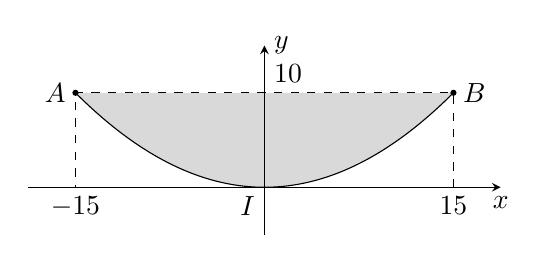
\begin{tikzpicture}[smooth,samples=300,scale=0.6,>=stealth]
\fill[gray!30] (-4,2)--(4,2)--plot[domain=4:-4](\x,{0.125*(\x)^2});
\draw[->] (-5,0)--(5,0) node[below]{$x$};
\draw[->] (0,-1)--(0,3) node[right]{$y$};
\draw (0,0) node[below left]{$I$};
\draw[domain=-4:4] plot(\x,{0.125*(\x)^2});
\draw[fill=black] (4,2) circle(1.5pt) (-4,2) circle(1.5pt);
\draw[dashed] (4,0)node[below]{$15$}--(4,2)node[right]{$B$}--(-4,2)node[left]{$A$}--(-4,0)node[below]{$-15$};

\node[right] at (0,2.4) {$10$};
\end{tikzpicture}}
\noindent
Vậy $y=\dfrac{2}{45}x^2$. Diện tích phần tô đen là $S=2 \cdot \displaystyle\int\limits_{-15}^{15} \left(10-\dfrac{2}{45}x^2 \right) \mathrm{\,d}x=400 \, (\text{m}^2)$.\\
Diện tích phần còn lại của sân bóng là $S_2=30 \cdot 50-400=1100\,(\text{m}^2).$\\
Số tiền Ông An phải trả để trồng cỏ nhân tạo cho sân bóng là
\[130000\times 400+90000\times 1100=151000000\text{ đồng}=151\text{ triệu đồng.}\]}
\end{ex}

\begin{ex}%[2H5C1-7]
Một phần sân nhà bác An có dạng hình thang $ABCD$ vuông tại $A$ và $B$ với độ dài $AB=9$ m, $AD=5$ m và $BC=6$ m như Hình 5.9. Theo thiết kế ban đầu thì mặt sân bằng phẳng và $A$, $B$, $C$, $D$ có độ cao như nhau. Sau đó bác An thay đổi thiết kế để nước có thể thoát về phía góc sân ở vị trí $C$ bằng cách giữ nguyên độ cao ở $A$, giảm độ cao của sân ở vị trí $B$ và $D$ xuống thấp hơn độ cao ở $A$ lần lượt là $6$ cm và $3{,}6$ cm. Để mặt sân sau khi lát gạch vẫn là bề mặt phẳng thì bác An cần phải giảm độ cao ở $C$ xuống bao nhiêu cm so với độ cao ở $A$?
\begin{center}
\includegraphics[scale=.4]{images/2P5-1-H5-9}
\hspace{0.5cm}
\begin{tikzpicture}[scale=0.5, font=\footnotesize,line join=round, line cap=round, >=stealth]
\path
(0,0) coordinate (A)
(9,0) coordinate(B)
(9,-6) coordinate(C)
(0,-5) coordinate(D)
;
\draw[thick] (A)--(B)--(C)--(D)--cycle;
\node [above] at ($(A)!0.5!(B)$) {$9$ m};
\node [right] at ($(B)!0.5!(C)$) {$6$ m};
\node [left] at ($(A)!0.5!(D)$) {$5$ m};
\foreach \i/\g in {A/90,B/90,C/-90,D/-90}{\draw[fill=black](\i) circle (0pt) ($(\i)+(\g:4mm)$) node[scale=1]{$\i$};}
\end{tikzpicture}
\end{center}
% \shortans{$10{,}32$}
\loigiai{
Tại vị trí ban đầu $A$, $B$, $C$, $D$ có độ cao như nhau, chọn hệ trục tọa độ có gốc tọa độ là điểm $A$ và các trục tọa độ lần lượt là $AD$, $AB$ và $Az$, với $Az \perp (ABCD)$.\\
Khi đó $A(0 ; 0 ; 0)$, $D(5; 0 ; 0)$, $B(0; 9 ; 0)$, $C(6; 9 ; 0)$.\\
Sau đó bác An thay đổi thiết kế để nước có thể thoát về phía góc sân ở vị trí $C$ bằng cách giữ nguyên độ cao ở $A$, giảm độ cao của sân ở vị trí $B$ và $D$ xuống thấp hơn độ cao ở $A$ lần lượt là $6$ cm và $3{,}6$ cm.\\
Khi đó, $A(0 ; 0 ; 0)$, $D(5; 0 ; -3{,}6)$, $B(0; 9 ; -6)$.\\
Ta có $\overrightarrow{AB}=(0 ; 9 ; -6)$, $ \overrightarrow{AD}=(5 ; 0 ; -3{,}6)$ là cặp véc-tơ chỉ phương của mặt phẳng $(ABD)$ nên một véc-tơ pháp tuyến của $(ABD)$ là $\left[\overrightarrow{AB}, \overrightarrow{AD}\right]=(-32{,}4 ; -30 ; -45)$.\\
Vậy mặt phẳng $(ABD)$ qua $A(0 ; 0 ; 0)$ và có véc-tơ pháp tuyến $\vec{n}=(-32{,}4 ; -30 ; -45)$ nên có phương trình là
\[-32{,}4 (x-2)-30(y+1)-45(z-3)=0 \qquad \text{hay } -32{,}4 x -30y -45z=0.\]
Để mặt sân sau khi lát gạch vẫn là bề mặt phẳng thì bác An cần phải giảm độ cao ở $C$ xuống $k$ centimét so với độ cao ở $A$ nên suy ra $C(6; 9 ; -k)$.\\
Ta có $A$, $B$, $C$, $D$ đồng phẳng	$\begin{aligned}[t]
&\Leftrightarrow C \in (ABD)\\
&\Leftrightarrow -32{,}4\cdot 6 -30 \cdot 9 -45\cdot (-k)=0\\
&\Leftrightarrow k=10{,}32.
\end{aligned}$\\
Vậy bác An cần phải giảm độ cao ở $C$ xuống $10{,}32$ centimét so với độ cao ở $A$.
}
\end{ex}
\Closesolutionfile{ans}


% \Closesolutionfile{ansbook}
% \HetDe
% \label{De3}
% %
% \cleardoublepage
% \setcounter{page}{1}
% \rfoot{Trang \thepage/\pageref{DA3} - Đáp án trắc nghiệm Mã đề 3}
% \begin{center}
% 	\bfseries ĐÁP ÁN TRẮC NGHIỆM MÃ ĐỀ 3
% \end{center}

% \inputansbox{10}{ans/ansDe3-TN1}
% \inputansbox[3]{2}{ans/ansDe3-TN2}
% \inputansbox{3}{ans/ansDe3-TN3}
% \label{DA3}
% %
